% chapter3_9.tex -- de (German)
% assigning RFID cards to audio files/folders
\section{Zuordnung von H�rspielen zu {\Karte}n }
\label{sect:assignment}

\begin{bclogo}[logo = \bclampe, noborder = true]{Hinweis}
Die funktionalen Elemente der {\Bezeichnung} sind nun installiert. Jetzt
ist es an der Zeit, einzelnen H�rspielen oder Musikst�cken {\Karte}n
zuzuordnen und einen \textit{Soundcheck} zu machen, um die grundlegende
Funktionalit�t der Box zu �berpr�fen:
\end{bclogo}

\begin{figure}[!h]
\centering

\includegraphics[width=0.45\textwidth]{/software/helloween.jpg}

\includegraphics[width=0.45\textwidth]{/software/metallica.jpg}
\caption{Audiodaten (Musikalben) auf die {\Bezeichnung} kopieren}
\end{figure}

Zun�chst werden \textit{rekursiv} zwei Unterverzeichnisse mit den
Musikdateien zweier Musikalben vom PC in den Audioordner auf der 
{\Bezeichnung} kopiert:\\
\cmdPC{scp -r Helloween pi@phoniebox1:/home/pi/RPi-Jukebox-RFID/shared/audiofolders}\\
\cmdPC{scp -r Metallica pi@phoniebox1:/home/pi/RPi-Jukebox-RFID/shared/audiofolders}

Kontrolle mit \cmd{ls -lR} auf der {\Bezeichnung}:\\
\cmdPi{ls -lR /home/pi/RPi-Jukebox-RFID/shared/audiofolders}
\begin{smaller}
\begin{verbatim}
total 26728
drwxr-xr-x 2 pi pi           4096 May 17 15:50  Helloween
drwxr-xr-x 2 pi pi           4096 May 17 15:56  Metallica

./Helloween:
total 104140
-rwxr-xr-x 1 pi pi 37314544 May 17 15:47 01_I_Want_Out.flac
-rwxr-xr-x 1 pi pi 38112711 May 17 15:48 02_Dr._Stein.flac
-rwxr-xr-x 1 pi pi 31203347 May 17 15:49 03_Future_World.flac

./Metallica:
total 151828
-rwxr-xr-x 1 pi pi 38978523 May 17 15:52 01_Enter_Sandman.flac
-rwxr-xr-x 1 pi pi 41647915 May 17 15:54 02_Sad_But_True.flac
-rwxr-xr-x 1 pi pi 29319722 May 17 15:54 03_Holier_Than_Thou.flac
-rwxr-xr-x 1 pi pi 45518619 May 17 15:56 04_The_Unforgiven.flac
\end{verbatim}
\end{smaller}

\subsection{{\Karte} manuell zuordnen}
Um nun diesen beiden Alben zwei neue {\Karte}n zuzuordnen, sind folgende
Schritte erforderlich:
\begin{compactitem}
\item{ID der neuen {\Karte} herausfinden}
\item{F�r jede ID die Shortcut-Datei nacheditieren.} 
%\item{Playlist als \cmd{*.m3u}-Datei erstellen} # braucht's nicht!
%%%%
%\item{F�r jede ID die Shortcut-Datei \filenam{/home/pi/RPi-Jukebox-RFID/shared/shortcuts/000???????} anlegen, in der der Name einer \cmd{*.m3u}-Datei eingetragen ist.} 
%\item{Im Verzeichnis \filenam{/home/pi/RPi-Jukebox-RFID/playlists} die \cmd{*.m3u}-Datei mit dem oben angegebenen Namen anlegen}
\end{compactitem}

Zun�chst wird eine neue {\Karte} �ber den {\reader} eingelesen. Dabei
wird im Unterverzeichnis \filenam{/home/pi/RPi-Jukebox-RFID/shared/shortcuts}
eine Datei angelegt, die den Namen der Karten-ID hat, \zB \cmd{0009563230}.
Der Inhalt dieser Datei muss auf den Verzeichnisnamen des Albums oder
H�rbuchs unter \filenam{/home/pi/RPi-Jukebox-RFID/shared/audiofolders}
angepasst werden, \zB "`Helloween"'.\\
\cmdPi{nano /home/pi/RPi-Jukebox-RFID/shared/shortcuts/0009563230}\\
\stdout{Helloween}

%\subsection{ID einer neuen {\Karte} ermitteln}
%Die ID einer {\Karte} wird beim Einlesen durch den {\reader} in der
%Datei \filenam{/home/pi/RPi-Jukebox-RFID/settings/Latest\_RFID} abgelegt.
%Nach erfolgtem Einlesen den Inhalt dieser Datei anzeigen:\\
%\cmdPi{cat /home/pi/RPi-Jukebox-RFID/settings/Latest\_RFID}\\
%\stdout{0009563230}
%
%\subsection{Shortcut-Datei f�r die soeben ermittelte ID anlegen}
%Im Unterverzeichnis \filenam{/home/pi/RPi-Jukebox-RFID/shared/shortcuts}
%wird eine Datei angelegt, deren Dateiname der ermittelten ID, \zB 
%\cmd{0009563230} entspricht. In dieser Datei wird der Name des
%Unterverzeichnisses des gew�nschten Albums in\\
%\filenam{/home/pi/RPi-Jukebox-RFID/shared/audiofolders} eingetragen, \zB
%"`Helloween"'.\\
%\cmdPi{nano /home/pi/RPi-Jukebox-RFID/shared/shortcuts/0009563230}\\
%\stdout{Helloween}
%
%\subsection{Playlist f�r dieses Album als \cmd{*.m3u}-Datei erstellen}
%Die Playlist, die bei Auflegen dieser Karte abgespielt werden soll,
%muss im Verzeichnis\\ \filenam{/home/pi/RPi-Jukebox-RFID/playlists} als
%\cmd{*.m3u}-Datei erstellt werden. Dabei handelt es sich einfachsten
%Fall um eine Textdatei, die in jeder Zeile eine abzuspielende Audiodatei
%enth�lt, siehe \url{https://de.wikipedia.org/wiki/M3U}:\\
%\cmdPi{nano /home/pi/RPi-Jukebox-RFID/playlists/Helloween.m3u}\\
%\stdout{/home/pi/RPi-Jukebox-RFID/shared/audiofolders/Helloween/01\_I\_Want\_Out.flac\\
%        /home/pi/RPi-Jukebox-RFID/shared/audiofolders/Helloween/02\_Dr.\_Stein.flac\\
%        /home/pi/RPi-Jukebox-RFID/shared/audiofolders/Helloween/03\_Future\_World.flac
%       }

Nach erneutem Auflegen der {\Karte} mit der ID \cmd{0009563230} werden
%die in der Playlist hinterlegten Musiktitel des Albums \textit{Helloween
%-- The Best, The Rest, The Rare} abgespielt.
die im Verzeichnis \filenam{/home/pi/RPi-Jukebox-RFID/shared/audiofolders/Helloween}
abgelegten Audiodateien abgespielt.

%\begin{bclogo}[logo = \bclampe, noborder = true]{Hinweis}
%Wichtig ist bei diesem Vorgehen, dass sowohl der Dateiname der
%Playlist als auch das Albumsverzeichnis genau der Bezeichnung aus der
%Shortcut-Datei entsprechen muss, hier also "`Helloween"'!
%\end{bclogo}

\subsection{{\Karte} �ber die Webanwendung registrieren}
Alternativ kann eine {\Karte} auch mit Hilfe des Webservices zugeordnet
werden. Das Vorgehen wird in der folgenden Bilderstrecke dargestellt:

\begin{figure}[!h]
\centering
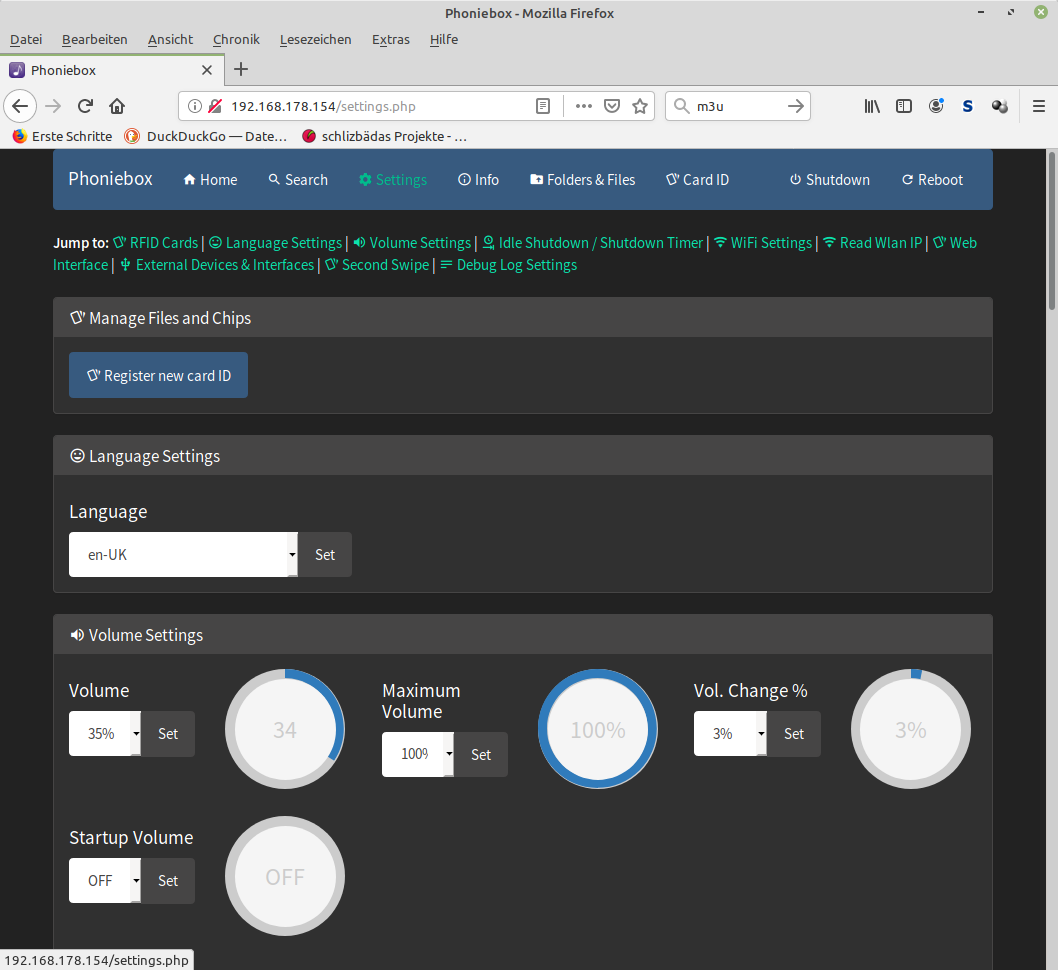
\includegraphics[width=0.49\textwidth]{/software/webservice-metallica01.png}
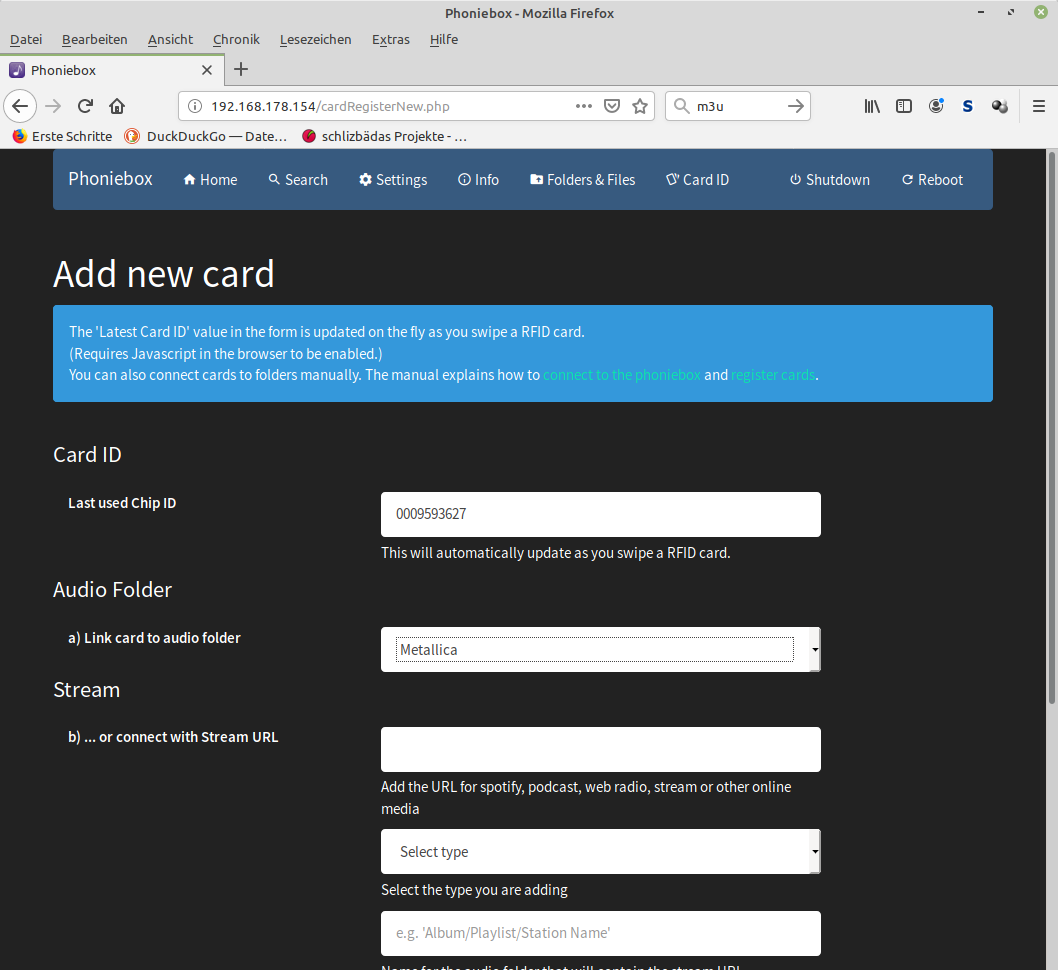
\includegraphics[width=0.49\textwidth]{/software/webservice-metallica02.png}
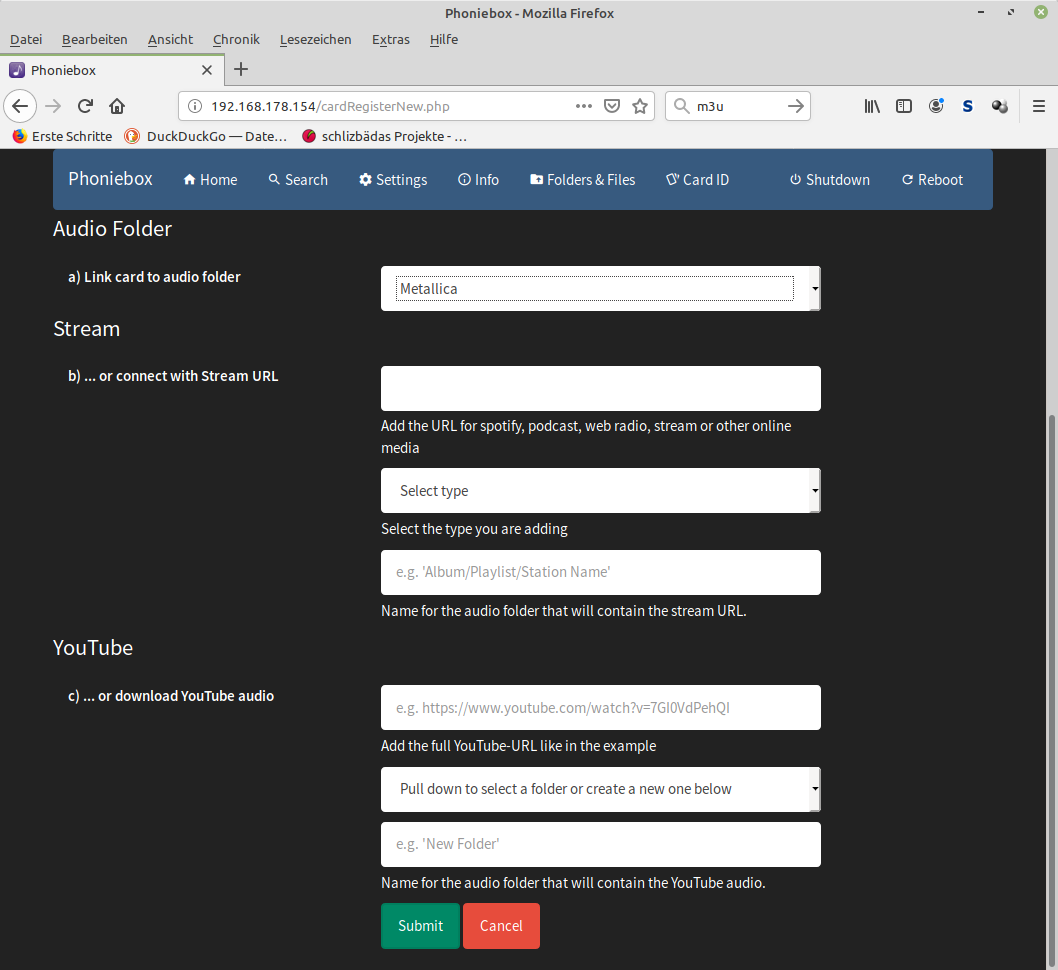
\includegraphics[width=0.49\textwidth]{/software/webservice-metallica03.png}
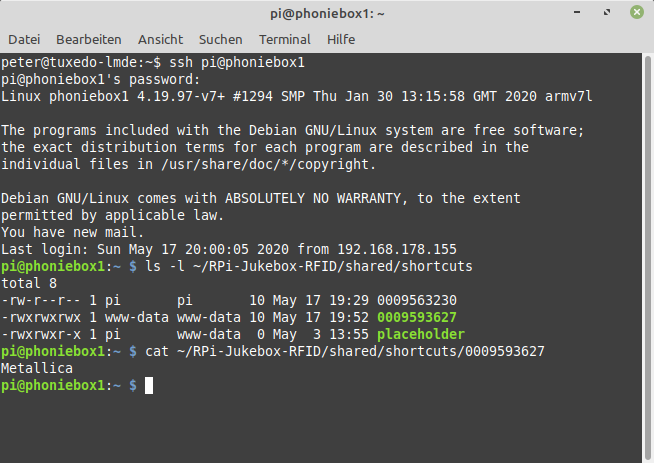
\includegraphics[width=0.49\textwidth]{/software/webservice-metallica04.png}
\caption{{\Karte} �ber Webservice registrieren}
\end{figure}

Am PC wird �ber einen Internetbrowser (Firefox) eine Verbindung zur
{\Bezeichnung} hergestellt, z.B. durch Eingabe der IP-Adresse (hier
192.168.178.154). Durch Klick auf \menuitem{Settings} in der oberen
Men�leiste erscheint das Bild links oben. Hier muss auf die Schaltfl�che
\button{Register new card ID} geklickt werden. Nun erscheint das Bild
rechts oben. Jetzt die neue {\Karte} �ber den {\reader} einlesen. Im
dazugeh�rigen Textfeld wird die ID aktualisiert (hier \cmd{0009593627}).

In der Zeile \menuitem{Audio Folder} werden im Auswahlfeld (ComboBox)
alle Unterverzeichnisse von \filenam{/home/pi/RPi-Jukebox-RFID/shared/audiofolders}
angezeigt. Hier den gew�nschten Ordner "`Metallica"' ausw�hlen. Zum
Speichern der gew�hlten Einstellungen im Browser nach unten scrollen
und die gr�ne Schaltfl�che \button{Submit} anklicken.

Eine �berpr�fung im ssh-Terminal zeigt die Zuordnung der neuen {\Karte}
zum Album "`Metallica"':\\
\cmdPi{cat ~/RPi-Jukebox-RFID/shared/shortcuts/0009593627}\\
\stdout{Metallica}

Auch hier bewirkt das erneute Auflegen dieser Karte den Start der
Wiedergabe der Audiodateien.

\subsection{Testen der Taster an den GPIO-Pins}
In der Konfiguration von {\autor}s {\Bezeichnung} sind in der Datei\\
\filenam{/home/pi/RPi-Jukebox-RFID/scripts/gpio-buttons.py} an folgenden
GPIOs Taster definiert, siehe auch Kapitel \ref{sect:prototypingboard}
sowie Tabelle \ref{tab:gpio_rpi}:

\begin{table}[!h]
\centering
\renewcommand{\arraystretch}{1.25}
\begin{tabular}{|p{0.10\textwidth}|p{0.10\textwidth}|p{0.15\textwidth}|p{0.30\textwidth}|p{0.20\textwidth}|}
\hline
\textbf{GPIO}	&	\textbf{Pin}	&	\textbf{Funktion}	&	\textbf{Beschreibung}	&	\textbf{Anmerkung}\\
\hline
\texttt{13}		&	\texttt{33}		&	\textit{vol0}		&	stumm schalten			&	(nicht verwendet)\\
\hline
\texttt{12}		&	\texttt{32}		&	\textit{volU}		&	Lautst�rke erh�hen		&\\
\hline
\texttt{6}		&	\texttt{31}		&	\textit{volD}		&	Lautst�rke verringern	&\\
\hline
\texttt{7}		&	\texttt{26}		&	\textit{next}		&	n�chster Titel			&\\
\hline
\texttt{8}		&	\texttt{24}		&	\textit{prev}		&	vorheriger Titel		&\\
\hline
\texttt{5}		&	\texttt{29}		&	\textit{halt}		&	Play/Pause				&\\
\hline
\end{tabular}
\vspace{0.5cm}
\caption{Taster an der GPIO-Leiste bei {\autor}s \Bezeichnung}
\label{tab:gpio_buttons}
\end{table}

Die Taster k�nnen bei dieser Gelegenheit auch gleich auf Funktion
�berpr�ft werden \smiley{smile}
